\chapter{github Actionsの設定}

githubActionsを設定していきましょう。

流れとしては、新しいブランチを作成して、その中にhugoを実行させて静的なファイルを作成して、強制プッシュを用いて更新をかけていくやり方です。
無理くり動かしている雰囲気は感じますが、今はこのままでいきましょう。
何かいい方法がありましたら、教えてください。

.github/workflowsフォルダーを作成しましょう
その中にgithub-actions-demo.ymlとして、ファイルを作成しておきましょう

\begin{shaded}
  \begin{verbatim}
  $ mkdir .github
  $ cd .github
  $ mkdir workflows
  $ cd workflows
  $ touch github-actions-demo.yml
  \end{verbatim}
\end{shaded}

\begin{figure}[H]
  \centering
  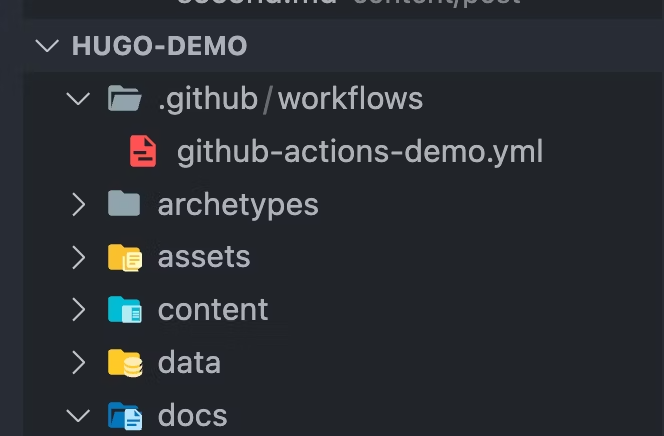
\includegraphics[width=8cm]{./image/02-chap8/make-github-workflow.png}
  \caption{github-actionsの設定ファイルを作成 }
  \label{chap8-make-github-workflow-image}
\end{figure}

中のファイルはこのように書き込んでいきましょう。
一部人によって変わる場所があるので気をつけてください。

** 変えるもの **
起爆させるブランチ名 コミットする時のユーザー名、ファイル名

\begin{tcolorbox}[breakable]
  \begin{verbatim}
    name: Deploy Sakura Server

    on:
      push:
        branches:
          - master  # masterブランチが更新された時に発火させる
    
    jobs:
      deploy:
        name: deploy
        runs-on: ubuntu-latest
        
        steps:
          - uses: actions/checkout@v2
            with:
              submodules: true  # Fetch Hugo themes (true OR recursive)
              fetch-depth: 0    # Fetch all history for .GitInfo and .Lastmod
    
          - name: Setup Hugo
            uses: peaceiris/actions-hugo@v2
            with:
              hugo-version: '0.102.3'  # コンパイルに使用するHugoのバージョンを指定
    
          - name: Build
            run: hugo --minify  # 実際にHugoでコンパイルする(--minifyはファイルを圧縮するオプション)
    
          - name: git commit
            uses: EndBug/add-and-commit@v9
            with:
              author_name: harutiro # 投稿するユーザーに合わせてください。
              author_email: hogehoge@example.com # 投稿するユーザーに合わせてください。
              new_branch: web_public
              message: 'hogehoge' # いい感じにメッセージを書いてあげてください。
              add: '* --force' 
              push: origin web_public --force
  \end{verbatim}
\end{tcolorbox}

あとは、新しくgithubpagesの設定を書き換えて完成です。
ブランチの位置をweb$\_$publicに書き換えましょう。

\begin{figure}[H]
  \centering
  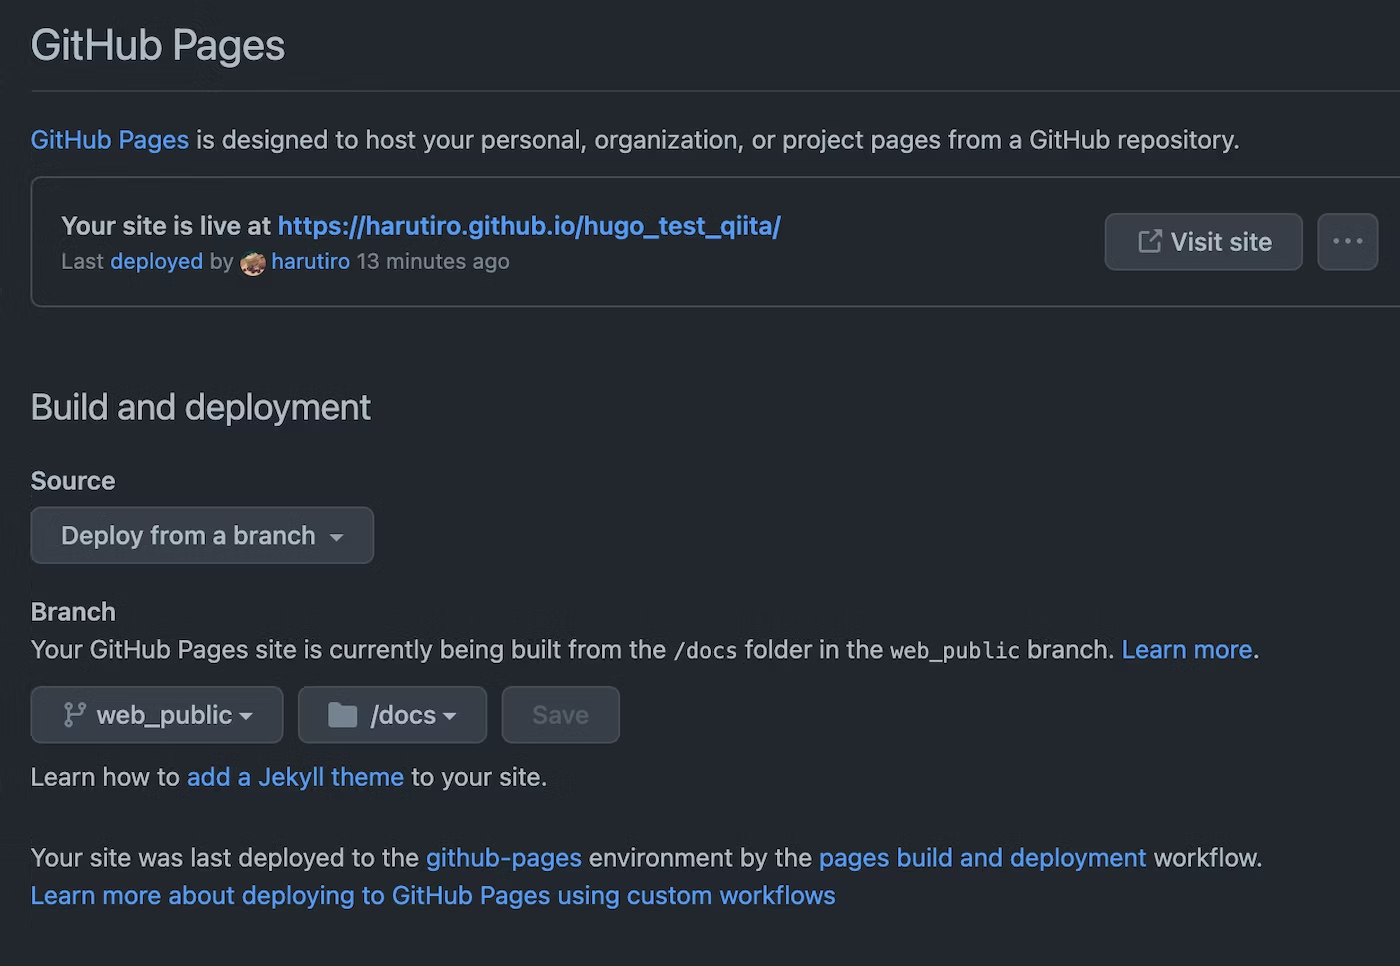
\includegraphics[width=8cm]{./image/02-chap8/web_public.png}
  \caption{github-pagesの設定を書き換える}
  \label{chap8-web_public-image}
\end{figure}

これで完成です。
新しくpushがされたタイミングで更新がかかっていきます。